\section{Capped hose model}
In this section, we now turn to a different class of (symmetric) demand matrices, referred to as the \emph{capped hose model}.
We can describe the capped hose model with linear constraints: each terminal $i$ has maximum capacity $b_i$ (as in the hose model), and additionally there is an upper bound $d_{ij}$ on the demand between terminals $i,j \in W$.
Hence, we can describe the capped hose polytope $\mathcal H^\text{cap}(b, d)$ as all (symmetric) matrices $(D_{ij})_{i,j \in W}$ for which
\[
    \begin{split}
        \sum_{j \in W} D_{ij} &\le b_i \qquad&&\forall_{i \in W}, \\
        D_{ij} &\le d_{ij} \qquad&&\forall_{i,j \in \binom W 2}.
    \end{split}
\]
Note that setting $d_{ij} = 0$ signals that terminals $i$ and $j$ may not communicate.

We define a graph $H$ with vertex set the terminals $W$ and edges $W \times W$, weighted with $d_{ij}$.
We will first derive a compact MIP formulation for general robust network design problems under the capped hose demand model.
We will then focus on the case where $H$ is a cycle, i.e.\ terminals are only allowed to communicate with its two direct neighbors in the cycle.
In this case, a dynamic programming algorithm is suggested by Bosman and Olver~\cite{bosman2017exploring}, for which it is shown that it is optimal when $b$ and $d$ are unit.
Optimality remains an open problem for arbitrary $b$ and $d$.

\subsection{MIP formulation}
As for the VPN and generalized VPN problem, we first write the semi-infinite MIP formulation with the row generation subproblems.
We then use a dualization trick to obtain a compact formulation.

Let $x_{uv}$ denote the amount of capacity we buy of edge $\{u,v\}$ in the network graph $G$.
The semi-infinite MIP formulation becomes
\begin{alignat*}{5}
    \text{minimize}\ && \sum_{uv \in E} c_{uv} \cdot x_{uv} &&& \\
    \text{subject to}\ && x_{uv} &\ge \sum_{ij \in \binom{W}{2}} D_{ij} \cdot (f_{uv}^{ij} + f_{vu}^{ij}) &&\qquad \forall_{uv \in E,\ D \in \mathcal U^*} \\
    && \sum_{uv \in \delta(u)} f_{uv}^{ij} - f_{vu}^{ij} &= \begin{cases}
                                                                1 & \text{if $u = i$} \\
                                                                -1 & \text{if $u = j$} \\
                                                                0 & \text{otherwise}
    \end{cases} &&\qquad \forall_{u \in V,\ ij \in \binom{W}{2}} \\
    && x_{uv} &\in \mathbb{R}_+ &&\qquad \forall_{uv \in E} \\
    && f_{uv}^{ij},\ f_{vu}^{ij} &\in \{ 0, 1 \} &&\qquad \forall_{uv \in E,\ ij \in \binom{W}{2}}
\end{alignat*}
where $\mathcal U^* \subseteq \mathcal H^\text{cap}(b, d)$, and is populated by solving the following row generation subproblems (for all $uv \in E$).
Let $(\tilde x, \tilde f)$ denote the current optimal solution of the master problem.
\begin{alignat}{5}
    \text{maximize}\quad && \sum_{ij \in \binom{W}{2}} (\tilde f_{uv}^{ij} + \tilde f_{vu}^{ij}) \cdot D_{ij} &&& \\
    \text{subject to}\quad && D_{ij} &\le d_{ij} &&\qquad \forall_{ij \in \binom W 2} \label{eq:cap:constr1}\\
    && \sum_{\substack{j \in W:\\i \neq j}} D_{ij} &\le b_i &&\qquad \forall_{i \in W} \label{eq:cap:constr2} \\
    && D_{ij} &\in \mathbb{R}_+ &&\qquad \forall_{ij \in \binom{W}{2}}
\end{alignat}
Let $D^*$ denote the optimal solution of the above row generation subproblem.
If the objective of $D^*$ violates the constraint in the master problem (when its greater than $\tilde x_{uv}$), then we add $D^*$ to $\mathcal U^*$.

\subsubsection{Compact formulation}
To obtain the compact formulation, we dualize the subproblems.
Fix an edge $uv \in E$.
We introduce dual variables $\psi_{ij}^{uv}$, for all $ij \in \binom W 2$, for the constraint~\eqref{eq:cap:constr1}, and $\omega_i^{uv}$ for all $i \in \binom W 2$, for constraint~\eqref{eq:cap:constr2}.
We then get the dual
\begin{alignat*}{5}
    \text{minimize}\quad && \sum_{ij \in \binom{W}{2}} d_{ij} \cdot \psi_{ij}^{uv} + \sum_{i \in W} b_i \cdot \omega_i^{uv} &&& \\
    \text{subject to}\quad && \psi_{ij}^{uv} + \omega_i^{uv} + \omega_j^{uv} &\ge f_{uv}^{ij} + f_{vu}^{ij} &&\qquad \forall_{ij \in \binom W 2} \\
    && \psi_{ij}^{uv} &\in \mathbb{R}_+ &&\qquad \forall_{ij \in \binom{W}{2}} \\
    && \omega_i^{uv} &\in \mathbb{R}_+ &&\qquad \forall_{i \in W}
\end{alignat*}
Because of strong duality and because $x_{uv}$ appears with nonnegative coefficients in the objective, we can substitute the dual into the master problem to obtain a compact formulation:
\begin{alignat*}{5}
    \text{minimize}\ && \sum_{uv \in E} c_{uv} \cdot x_{uv} &&& \\
    \text{subject to}\ && x_{uv} &\ge \sum_{ij \in \binom{W}{2}} d_{ij} \cdot \psi_{ij}^{uv} + \sum_{i \in W} b_i \cdot \omega_i^{uv} &&\qquad \forall_{uv \in E} \\
    && \psi_{ij}^{uv} + \omega_i^{uv} + \omega_j^{uv} &\ge f_{uv}^{ij} + f_{vu}^{ij} &&\qquad \forall_{uv \in E,\ ij \in \binom W 2} \\
    && \sum_{uv \in \delta(u)} f_{uv}^{ij} - f_{vu}^{ij} &= \begin{cases}
                                                                1 & \text{if $u = i$} \\
                                                                -1 & \text{if $u = j$} \\
                                                                0 & \text{otherwise}
    \end{cases} &&\qquad \forall_{u \in V,\ ij \in \binom{W}{2}} \\
    && x_{uv} &\in \mathbb{R}_+ &&\qquad \forall_{uv \in E} \\
    && \psi_{ij}^{uv} &\in \mathbb{R}_+ &&\qquad \forall_{uv \in E,\ ij \in \binom{W}{2}} \\
    && \omega_i^{uv} &\in \mathbb{R}_+ &&\qquad \forall_{uv \in E,\ i \in W} \\
    && f_{uv}^{ij},\ f_{vu}^{ij} &\in \{ 0, 1 \} &&\qquad \forall_{uv \in E,\ ij \in \binom{W}{2}}
\end{alignat*}

For the specific case where the support of $(d_{ij})$ is a cycle, an optimal dynamic programming algorithm is introduced in \cite{bosman2017exploring}, but it remains open whether it is optimal for arbitrary $b$ and $d$.
We discuss this algorithm next.

\subsection{The hubbing algorithm}
To obtain a dynamic programming algorithm, we first consider a slightly modified demand cycle graph $H$.
The cycle $H$ is modified by adding an extra vertex between each terminal and the cycle.
The resulting graph is denoted with $\hat H$ and the new vertex adjacent to terminal $v$ in $\hat H$ is denoted with $\hat v$ (see Figure~\ref{fig:hdak}).
Although we consider arbitrary $b$ and $d$, we do not lose any generality by restricting ourselves to the situation where the capacities are minimal, i.e.\ cannot be reduced while keeping the problem the same.
More concretely, this means that the capacity of an edge is not more than the capacity of an adjacent vertex, and the capacity of a vertex is not more than the sum of the capacities of the two adjacent edges.

\begin{figure}
    \centering
    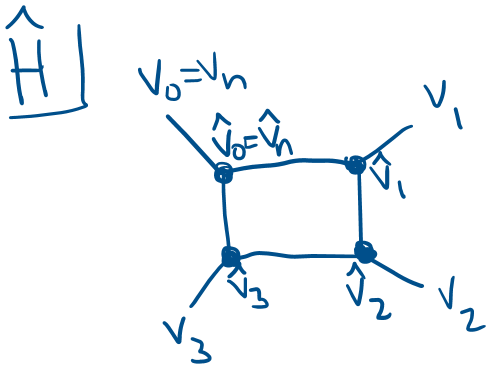
\includegraphics[width=.35\textwidth]{hdak.png}
    \caption{The graph $\hat H$.} \label{fig:hdak}
\end{figure}

Let the vertices on cycle $H$ be $v_0, v_1, \dots, v_n = v_0$.
Then the subproblem is defined in the following way: let $C[i, j, h(i), h(j)]$ be the minimum cost of only the part from $i$ to $j$ in $H$ (clockwise), where $\hat v_i$ is mapped to $h(i)$ and $\hat v_j$ is mapped to $h(j)$.
Here, $0 \le i < j \le n$ and all terminals must be mapped to itself.

If $j = i + 1$, then the cost is $b_i \cdot d_c(v_i, h(i)) + d_{ij} \cdot d_c(h(i), h(j)) + b_j \cdot d_c(v_j, h(j))$.
Here, $d_c(u, v)$ is the shortest path under cost function $c$ from $u$ to $v$ in $G$, i.e.\ buying each edge on the shortest path once.
It is considers the edge $\{\hat v_i, \hat v_j\}$ in the cycle in $\hat H$ and the two edges between these nodes and the corresponding terminals.
Because we required the capacities to be minimal, we know that there exist valid demands that utilize the full capacity.
Thus, we must buy these.

If $j$ is not $i+1$, we pick a node $\hat v_k$ with $i < k < j$ (for example, $k = i + 1$).
Then, $C[i, j, h(i), h(j)]$ is the minimum over all possible mappings $h(k) \in V_G$ of $C[i, k, h(i), h(k)] + C[k, j, h(k), h(j)] - b_k d(v_k, h(k))$.
Both parts consider the edge $(v_k, \hat v_k)$, so we should remove it once to obtain the correct answer.
See also Figure~\ref{fig:dp} for a sketch of the situation.

\begin{figure}
    \centering
    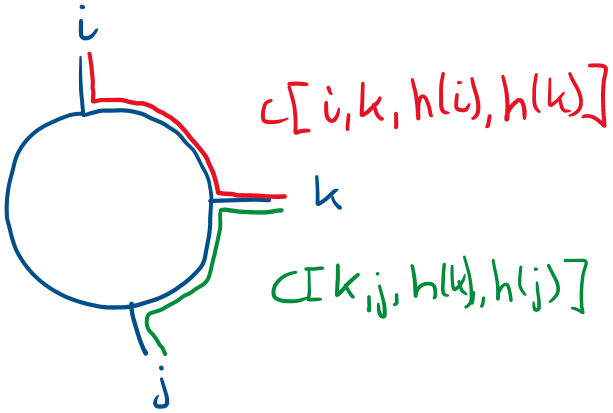
\includegraphics[width=.35\textwidth]{dp.png}
    \caption{Sketch of the situation for the dynamic program (in $\hat H$).} \label{fig:dp}
\end{figure}

This leads to the following recurrence:
\[
    C[i, j, h(i), h(j)] = \begin{cases}
                              0 &\text{if $i \ge j$} \\
                              b_i \cdot d_c(v_i, h(i)) + d_{ij} \cdot d_c(h(i), h(j)) + b_j \cdot d_c(v_j, h(j)) &\text{if $j = i+1$}\\
                              \displaystyle \min_{h(k) \in V_G} \{ C[i, k, h(i), h(k)] + C[k, j, h(k), h(j)] - b_k d(v_k, h(k)) \} &\text{otherwise}\\


    \end{cases}
\]

We can now determine all values by first determining the base cases, then all valid intervals of length two, then length three etc.
The last interval will go from $0$ to $n$ and this is the interval we are interested in.
The minimum over all mappings $h(0)$ of $C[0, n, h(0), h(0)]$ will be the minimum cost.
The actual mappings can be obtained by searching the table backwards.

%\subsection{Experiments}
%Experiments with integrality gap.

\subsection{Proving optimality of the hubbing algorithm in the cycle case}
In this section, we explore an approach to generalize the proof in \cite{bosman2017exploring} that the hubbing programming algorithm is optimal when $H$ is a cycle and $b$, $d$ unit, to our setting where $b$ and $d$ are arbitrary.

The original proof first shows that there is always an optimal solution with a certain nice structure, but is not quite yet a hubbing solution.
A last, rather non-trivial step of the proof shows that this structure can in fact be transformed to a hubbing solution.


To obtain this first structured optimal solution, it is first shown that we can restrict ourselves solutions of the compact MIP formulation where the (originally dual) variable from the row subproblem is integral.
We now show that we can extend this integrality assumption to our case as well, in particular, we will show that we can restrict to solutions where $\omega$ and $\psi$ in our compact formulation are integral.
We are now slightly adapting the notation from the previous sections to match with \cite{bosman2017exploring}: for an edge $e = \{u, v\}$ we now write $\omega_i(e)$ and $\psi_{ij}(e)$ instead of $\omega_i^{uv}$ and $\psi_{ij}^{uv}$.

\subsubsection{Rephrashed version of the problem}
In order to show this, we first write an expression for the minimum capacity we are required to buy for each edge, if we consider the routing template to be given.
The required capacity for an edge $e \in E(G)$ becomes
\[
    x(e) = \max_{D \in \mathcal H^\text{cap}(b, d)} \sum_{\substack{ij \in \binom W 2 :\\e \in P_{ij}}} D_{ij}.
\]
The resulting solution has cost $\sum_e c(e) x(e)$, and this we wish to minimize.

We can also formulate the dual version of the above, from which we obtain a convenient rephrased version of the problem.
The dual is formulated as
\[
    \begin{split}
        x(e) = \min \quad & \sum_{i \in W} b_i \omega_i(e) + \sum_{ij \in \binom W 2} d_{ij} \psi_{ij}(e) \\
        \text{s.t.}\quad & \omega_i(e) + \omega_j(e) + \psi_{ij}(e) \ge 1 \qquad \forall_{ij \in E(H) : e \in P_{ij}} \\
        & \omega_i(e),\ \psi_{ij}(e) \ge 0.
    \end{split}
\]
We then rephrase the problem as follows.
Each terminal $i$ `buys' a capacity vector $\omega_i$, and each connection $ij$ `buys' a capacity vector $\psi_{ij}$ (indexed by the edges $e \in E$ of $G$), with the property that $\{ e \in E : \omega_i(e) + \omega_j(e) + \psi_{ij}(e) \ge 1 \}$ contains an $i$--$j$-path, for each connection $ij \in E(H)$.
The goal is to minimize the total cost
\[
    \sum_{e \in E} c(e) u(e) = \sum_{i} b_i c(\omega_i) + \sum_{ij} d_{ij} c(\psi_{ij}),
\]
where $c(\omega_i) = \sum_{e \in E} c(e) \omega_i(e)$ and $c(\psi_{ij}) = \sum_{e \in E} c(e) \psi_{ij}(e)$ (one can verify the total cost expression by substituting the dual objective for $u(e)$, merging the ``min''s, and re-arranging the summations).

\subsubsection{Integral solutions}
We will show that Lemma~4 of \cite{bosman2017exploring} generalizes to our case, i.e.\ that we can restrict to integral capacity vectors $(\boldsymbol \omega, \boldsymbol \psi)$.
\begin{proof}
    First, note that in any optimal, possibly fractional, solution, we have that $0 \le \omega_i, \psi_{ij} \le 1$, by the nature of the dual formulation.
    Hence, if the solution is integral, we know that the capacity vectors are binary.
    It is convenient to express the solution as a collection of edge sets (which we denote with a capital letter) $\boldsymbol \Omega = (\Omega_i)$ and $\boldsymbol \Psi = (\Psi_{ij})$, where $\Omega_i = \{ e : \omega_i(e) = 1 \}$ and $\Psi_{ij} = \{ e : \psi_{ij}(e) = 1 \}$, i.e.\ the edges that each terminal/connection buys.

    We now assume that $H$ is a cycle, and show that there always exists an integral optimum solution to the capped hose problem.
    Notice that $u(e)$ is phrased as a fractional $d$-capacitated $b$-matching problem on $H$, which has an integral optimal solution if $H$ is bipartite (since the constraint matrix is the incidence matrix of $H$, which is totally unimodular, see also \cite{schrijver2003combinatorial} Theorem~21.8).
    Hence, if $H$ is an even cycle, it is bipartite and we are done.

    Now, consider the case when $H$ is an odd cycle.
    Since any strict subgraph of a cycle is bipartite, the only case where we do not have an integral optimal solution is when $u(e)$ corresponds to the dual $d$-capacitated $b$-matching problem on the complete cycle.
    This only happens if the routing path between \emph{every} pair of neighbors uses the edge.

    So suppose $e = \{u, v\}$ is used on every routing path $P_{ij} \in \mathcal P$.
    Let $(\boldsymbol \omega, \boldsymbol \psi)$ a (possibly fractional) dual solution, with corresponding primal solution $D$.
    We first assume that this solution saturates $b$, i.e.\ the optimal primal solution $D$ satisfies
    \[
        D_{i-1,i} + D_{i,i+1} = b_i
    \]
    for all $i \in W$.
    We claim that the integral solution $(\boldsymbol Y, \boldsymbol Z)$, given by:
    \begin{itemize}
        \item taking $Y_i$ to be the set of edges of a shortest $i$--$v$-path (for all terminals $i$),
        \item taking $Z_{ij} = \varnothing$,
    \end{itemize}
    costs no more than $(\boldsymbol \omega, \boldsymbol \psi)$.

    The following closely resembles the arguments from \cite{bosman2017exploring}.
    We let $D$ be the traffic matrix from the primal solution.
    If we now route $D$ according to $(\boldsymbol \omega, \boldsymbol \psi)$, the flow between $i$ and $i+1$ can be split into flow between $i$--$v$ and flow between $v$--$(i+1)$, since every routing path passes through $e$, and thus through $v$.

    So $D$ induces a $i$--$v$ flow for each $i \in W$ of at least $b_i$, following directly from the fact that $b$ is saturated.
    So $(\boldsymbol \omega, \boldsymbol \psi)$ has sufficient capacity to route $b_i$ unit of flow from each $i \in W$ simultaneously.
    This costs at least as much as buying $b_i$ of every edge on a shortest path from terminal $i$ to $v$, for all terminals.
    The latter is exactly the cost of the integral solution $(\boldsymbol Y, \boldsymbol Z)$, proving the claim.

    We are left with the case where $\boldsymbol b$ is not saturated.
    We show that this is equivalent with a fractional capacitated $b$-matching problem on a path, which is bipartite and therefore shows that the solution is integral.

    As $\boldsymbol b$ is not saturated, there exists a terminal $i \in W$ such that
    \[
        D_{i-1,i} + D_{i,i+1} < b_i.
    \]
    By complementary slackness, we must have $\omega_i(e) = 0$.
    Construct now a new (fractional) $d'$-capacitated $b'$-matching problem on the graph $H'$ obtained from $H$ after `splitting' vertex $i$ (see Figure~\ref{fig:split}, which is much clearer than the formal definition in the next sentence).
    Thus, $H$ has vertex set $W\setminus \{i\} \cup \{i', i''\}$ and edge set $E(H') = E(H) \setminus \{ \{i-1,i\}, \{i, i+1\} \} \cup \{ \{i-1, i'\}, \{i'', i+1\} \}$.
    Set the connection capacities $d'_{i-1,i'} = d_{i-1,i}$, $d'_{i'',i+1} = d_{i,i+1}$ and $d'_{u,v} = d_{u,v}$ for pairs $uv$ not involving $i$, $i'$ or $i''$.
    Set the terminal capacities $b'_{i'} = b'_{i''} = \infty$ and $b'_j = b_j$ otherwise.

    \begin{figure}
        \centering
        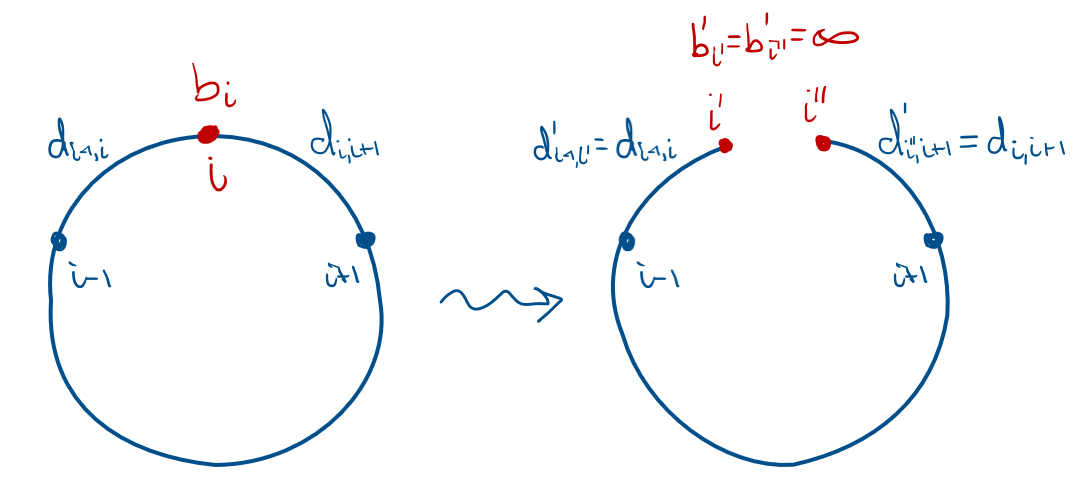
\includegraphics[width=.65\textwidth]{split}
        \caption{Construction of a new bipartite instance.} \label{fig:split}
    \end{figure}

    Note that the $(\boldsymbol \omega, \boldsymbol \psi)$ corresponds to a feasible dual solution $(\boldsymbol \omega', \boldsymbol \psi')$ in the constructed problem for $H'$, by setting $\omega'_{i'} = \omega'_{i''} = 0$.
    Note that the cost for both solutions are equal.
    We now argue that the constructed solution is optimal.
    We first observe that any optimal solution must have $\omega'_{i'} = \omega'_{i''} = 0$, as otherwise the objective becomes $\infty$.
    If there would exist a different solution with strictly smaller objective, this would correspond to a solution in the original problem with the same (strictly smaller) objective, contradicting optimality of $(\boldsymbol \omega, \boldsymbol \psi)$.
    Hence, $(\boldsymbol \omega', \boldsymbol \psi')$ is integral as $H'$ is bipartite, and hence $(\boldsymbol \omega, \boldsymbol \psi)$ is integral as well.
\end{proof}

\subsubsection{Integrality gap instances}
The proof is useful as an extension of Lemma~4 from \cite{bosman2017exploring}.
For the compact MIP formulation above, this proof shows that if we can assume $f$ is integral, then this implies that $\omega$ and $\psi$ are also integral.
Also the reverse implication holds, as for fixed integer $\omega$ and $\psi$ the problem reduces to a multicommodity flow problem with integer capacities.
This does not mean, however, that the whole formulation is integral.
Indeed, there exist instances for which an integrality gap is present, even for the case where $b$ and $d$ are unit.
These instances are the natural extension of integrality gap instances identified for the VPN problem and presented in \cite{goyal2013vpn}.
The largest integrality gap we found is using the graph with $4$ terminals in Figure~\ref{fig:gap4}, where the cycle is defined by unit $b$ and $d$.
This instance gives an integrality gap of $9/8$, which is the same integrality gap as found for the VPN problem.
To the best of our knowledge, integrality gap instanced for the capped hose problem where $H$ is a cycle have not been identified before.

\begin{figure}
    \centering
    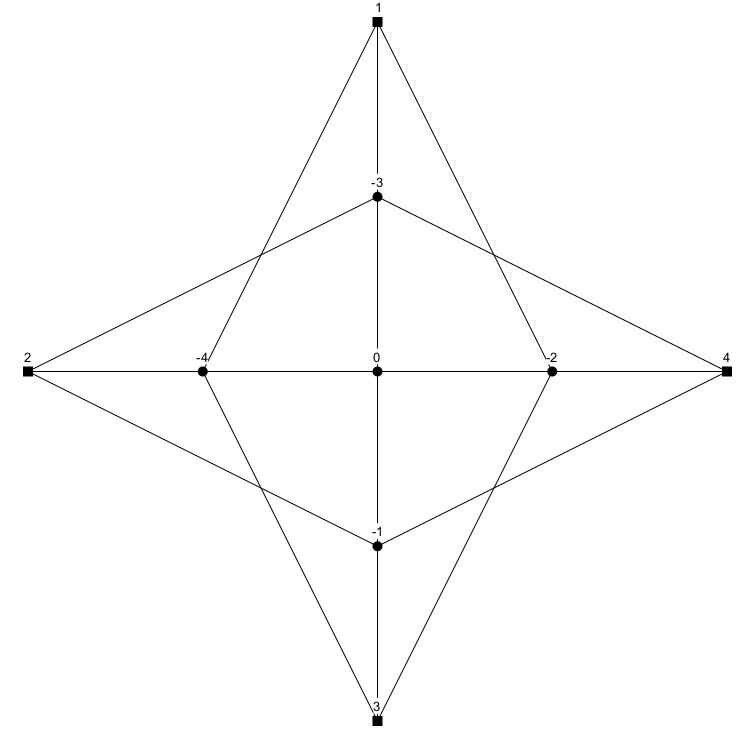
\includegraphics[width=.45\textwidth]{gap4}
    \caption{Integrality gap of $9/8$.} \label{fig:gap4}
\end{figure}

\subsubsection{Generalizing further}
It remains open whether it is possible to generalize the rest of the proof any further, as there are some challenges still to overcome there.
In short, the setup in definition~5 in \cite{bosman2017exploring} generalizes---maybe quite surprisingly---almost directly.
The partition of the mentioned feasible solution $\bar{\boldsymbol X}$ into sets $\bar{\boldsymbol X}_i$ and $\bar{\boldsymbol X}_{i,i+1}$ will intuitively correspond to the edges that are bought by terminals and connections, respectively.
We expect however that problems will arise in the proofs of lemma~11 and lemma~13, as here a solution $\bar{\boldsymbol X}$ is transformed into a different solution $\bar{\boldsymbol Y}$ by possibly switching edges from being bought by a terminal to being bought by a connection (or vice versa).
We make this clear with the following intuitive but very informal argument.
When being careful how many edges are switched, the cost of the resulting solution will not increase in the case where $b$ and $d$ are unit: you pay the same price for capacity regardless of whether the edge is bought by a terminal or a connection.
For arbitrary $b$ and $d$ this is no longer the case, and switching `buyers' of edge capacity might increase the total cost of the solution.
Luckily, the requirement that $b$ and $d$ are minimal gives some restriction on how much the cost can increase, but it is not immediately clear that the proofs of lemma~11 and lemma~13 will generalize.
